\section{Implementing a regular expression engine}
\label{sec:implementation}
The task of implementing a regular expression engine can be undertaken
in steps. The first steps is converting the regular expression to a
NFA. The next step is to simulate the NFA. The last step in our
implementation is to build filters.

%% \subsection{Datastructures}

%% \subsubsection{Representing the NFA}

%% For the representation of the NFA we started out as Russ Cox in
%% \cite{RussCox}. The NFA is represented as a linked collection of
%% \lstinline{State} structures:
%% \begin{lstlisting}
%% struct State
%% {
%%     unsigned int c;
%%     unsigned int type;
%%     struct State *out0;
%%     struct State *out1;
%% };
%% \end{lstlisting}
%% This is the essential contents of the \lstinline{State} structure. It
%% actually contains more variables, these will be added and explained
%% when appropriate. There is no explicit representation of the
%% transitions, they are represented as the two \lstinline{out} pointers in
%% the \lstinline{State} structure. The \lstinline{type}-variable decides the
%% type of the state and the transition(s):
%% \begin{description}
%% \item[split] This state is a split-state, both the two
%%   \lstinline{out}-pointers will be set to valid states.
%% \item[accepting] This is the accepting state.
%% \item[literal] This state only has a valid transition on the
%%   \lstinline{out0}-pointer. It is marked with the value in \lstinline{c}
%% \item[range] This is a state with a range-transition. These will
%%   be explained later in \vref{sec:ranges_impl}.
%% \item[epsilon] The transition in \lstinline{out0} is a
%%   $\upvarepsilon$-transition.
%% \end{description}



\subsection{Regular expression to NFA}

The first step in our regular expression engine is the regular
expression to NFA converter. As discussed in section
\vref{sec:re2nfa_thompson_theory}, the NFA is built from the regular
expression in steps from smaller NFA fragments. In order for this
method, used directly, to be successful, the regular expression has to
be in a form where the meta characters and the literals are presented
in the right order. Regular expressions with for example
\textsf{\textbar} can not simply be read from left to right and be
converted correctly. The problem with the alternation operator is that
it is an infix operator, so we only have the left hand side and not
the right hand side when we read the \textsf{\textbar} and can
therefore not complete the fragment.

Converting the regular expression to reverse polish notation, with an
explicit concatenation operator, or making a parse tree will solve
these problems. For this project neither is chosen. A third solution
to this problem is maintaining a stack where fragments and operators
are pushed and popped. This is the method that is implemented. We
tried determining the quality of the decision by comparing run times
with Russ Cox's example code \cite{Cox2007}. This did not go well due
to several reasons. The main reason is that the example code does not
do well on large examples\footnote{There are constants in the source
  code and a naive list append function} and large examples is needed
to do a reasonable comparison.

We followed Russ Cox' method from \cite{RussCox}, when converting the
regular expression to NFA. Russ Cox rewrites the regular expression to
reverse polish notation with an explicit concatenation operator, so
some changes will be necessary. There are tree main areas that needs
to be changed:

\begin{description}
\item[Concatenation] While constructing the NFA, NFA fragments are
  pushed onto a stack. Whenever the concatenation operator is
  encountered, the two top fragments are popped and patched together,
  see figure \vref{fig:concatenation}. We do not have the advantage of
  an explicit concatenation operator. Instead we will be trying to pop
  the top two NFA fragments and patching them together as often as
  possible. As often as possible is after a character is read, but
  before any action is taken on the character read. The exception to
  this rule is the quantifiers, which binds tighter than
  concatenation.
\item[Parentheses] The binding of the operators can be changed with
  parentheses. Not using a tree structure or reverse polish notation
  with an explicit concatenation operator, there is nothing showing
  the structure of how everything binds when simply reading the
  regular expression from left to right. We need some way of
  connecting the left parentheses to the matching right
  parentheses. For this we will be using the stack, we will expand it
  to also accept operators. Every time we read a left parenthesis in
  the regular expression, a left-parenthesis-fragment is pushed onto
  the stack. When we later on read a right parenthesis we simply pop
  fragments of the stack and patch them together till we reach a
  left-parenthesis-fragment.   
\item[Alternation] When reading the regular expression left to right,
  we only have the left NFA fragment ready when reading the
  alternation operator. Therefore we simply push the alternation
  operator on the stack. Whenever possible we pop the alternation
  operator and associated NFA fragments and patch them together, see
  figure \vref{fig:alternation}. This is probably not very often, as
  it will only happen after reading a right parenthesis or the end of
  the regular expression.
\end{description}


%% While constructing the NFA
%% we maintain a stack of NFA fragments. Each fragment consists of a
%% \lstinline{start} state and a list of its outgoing or dangling arrows:
%% \begin{lstlisting}
%% struct Fragment 
%% {
%%   unsigned int op;
%%   struct State *start;
%%   struct Statelist *out;
%% };
%% \end{lstlisting}
%% Here we see the first change: The \lstinline{op}-variable. This is
%% used when pushing operators on the stack. The two operators we need to
%% push is alternation and left parenthesis, so the possible values of
%% the \lstinline{op}-variable are:
%% \begin{description}
%% \item[none] This is a \lstinline{Fragment} representing a partial
%%   NFA. All \lstinline{Fragment}s with a value different from none, are
%%   not representing partial NFAs, they are merely markers.
%% \item[alternate] This \lstinline{Fragment} is a alternate marker.
%% \item[left parenthesis] This \lstinline{Fragment} is a left
%%   non-capturing left parenthesis marker.
%% \item[left capturing parenthesis] This \lstinline{Fragment} is a left
%%   capturing parenthesis marker.
%% \end{description}
%% In \cite{RussCox} Russ Cox does not need to push operators on the
%% stack, because they appear in the regular expression in the right
%% order. We need to somehow remember we have seen alternate and left
%% parenthesis operators, and the way we do this is to push them on the
%% stack. 

We have two important helper functions: \lstinline{maybe_concat} and
\lstinline{maybe_alternate}. The first concatenates the top two
fragments if possible, also see figure \vref{fig:concatenation}. The
second alternates the top fragments, if possible, so also figure
\vref{fig:alternation}. \lstinline{maybe_alternate} will pop alternate
markers from the stack. These are called as often as possible to keep
the stackdepth at a minimum and to avoid postponing all the
concatenating and alternating till the end. Supplying a regular
expression consisting entirely of left parenthesis will still make the
stackdepth grow to a maximum.

%% Whenever we encounter a right parenthesis we pop fragments of the
%% stack till we reach the left parenthesis marker fragment. The amount
%% of fragments we need to pop should not exceed one fragment after a
%% call to the helper functions \lstinline{maybe_concat} and
%% \lstinline{maybe_alternate}. If the parenthesis is empty we put in a
%% $\upvarepsilon$-transition. This is done because empty parenthesis is
%% often used instead of the empty string, which is very hard to write
%% explicitly seeing as it is empty.

\subsubsection{Character classes}
\label{sec:ranges_impl}

\begin{figure}
  \centering 
  \subfigure[\textsf{[a-c]}]{
    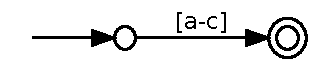
\includegraphics{implementation/range1.pdf}
    \label{fig:range1}
  }
  \subfigure[\textsf{a\textbar b\textbar c}]{
    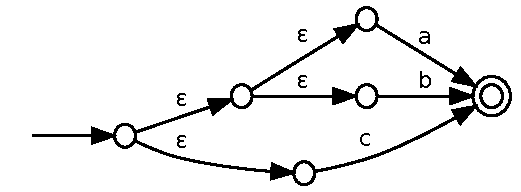
\includegraphics{implementation/range2.pdf}
    \label{fig:range2}
  }
  \caption{A simple character class-transition example}
  \label{fig:ranges}
\end{figure}

Character classes are part of the extension we made to the regular
expression definition. When implementing, we have the choice of
rewriting character classes in terms of the original regular
expressions, but as we can see in figure \vref{fig:ranges}, this
quickly becomes unwieldy. When we rewrite we add almost two states per
character matched by the character class, instead of adding just one
state for the whole character class. What we want is a NFA similar to
figure \ref{fig:range1}, not figure \ref{fig:range2}.

There are several ways of obtaining this goal. Perl uses a bitmap to
indicate membership of a range, for each character in the character
set there is a bit in the bitmap. To decide membership the bit
corresponding to the character is looked up. RE2 uses a balanced
binary tree, each node in the tree corresponds to either a whole range
or a literal character, the tree is then searched when deciding
membership. Each method has its advantages and drawbacks. The bitmap
is of constant size, so for small character classes, it will be
unnecessarily large, but the time to look up a value in the bitmap is
also constant and very fast. The balanced binary tree, has its
advantages for character classes with few ranges and literal
characters, since it will then be small in size and look up times. The
drawbacks are of course that it grows in size and look up times with
the character class.

For this project an even simpler solution was chosen: A simple linked
list of ranges. The literal characters will be represented as ranges
of length one. On other words, we will have one linked list per
character class, and the number of elements in each linked list is the
number of literals and ranges in the character class. Worst case we
will have to look through all members of a linked list to decide
membership of a character class. This is simplistic, but sufficient.

%% There should not be any serious
%% performance issues for simple character classes with few ranges and
%% literal characters.
%% \begin{lstlisting}
%% struct Range 
%% {
%%   unsigned int lo;
%%   unsigned int hi;
%%   struct Range *next;
%% };
%% \end{lstlisting}
%% The two unsigned integers are used to store the beginning and end of
%% the range, in the case of a single literal they are the same. The
%% \lstinline{next}-pointer points to the next range in the list. A
%% \lstinline{Range}-pointer and a flag to indicate whether or not the
%% character class is negated is added to the \lstinline{State} struct.

\subsection{The simulator}

We have built the NFA and the next step is to simulate it. This
requires keeping track of a set of active states. In a basic
implementation of the Thompson simulation algorithm
\cite{Thompson1968}, a state is only added to the active set
once. This will throw away matches, e.g. when the regular expression
\textsf{a\textbar a} is matched with the string \textsl{a} there are
two possible routes through the NFA, but only one will be reported,
since the final state will only be added once to the set of active
states.

We had to adjust the basic implementation to our needs; we need to
generate mixed bit-values. 

We implemented the standard Thompson algorithm for simulating a
NFA. It is important to note that this will throw away matches because
we only once add a state to the active set. There are however at least
two good reasons why you should not add a state more than once:
\begin{itemize}
\item Unless you are careful this will give rise to infinite loops in
  the simulation process. More on this below.
\item We open up for an exponential worst-case behavior. A good
  example is the same as the backtracking engine worst-case
  \textsf{a?$^n$a$^n$} matched with \textsl{a$^n$}. 
\end{itemize}

The problems with the infinite loops arise when matching with regular
expressions like \textsf{()*}, see figure \vref{fig:inf_loop_simple}
for the NFA. The simulator will go into a infinite loop generating
these bit-values:
\begin{verbatim}
  =0=0=0=0=0=0=0=0=0=0=0=0=0=0=0=0=0=0=0...
\end{verbatim}
This is because there is a cycle of $\upvarepsilon$-transitions in the
NFA. This would not be desirable behavior and we would need to stop
the simulation before it goes into an infinite loop. Note that this is
not implemented, as the problems with the infinite loops are not
applicable in a standard Thompson simulation.

\begin{figure}
  \centering \subfigure[\textsf{()*}]{
    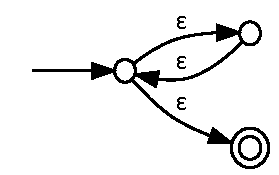
\includegraphics{implementation/inf_loop_simple.pdf}
    \label{fig:inf_loop_simple}
  }
  \subfigure[\textsf{(()())*}]{
    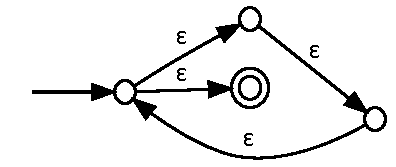
\includegraphics{implementation/inf_loop_long.pdf}
    \label{fig:inf_loop_long}
  }
  \subfigure[\textsf{(\textbar )*}]{
    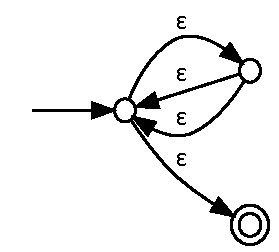
\includegraphics{implementation/inf_loop_many.pdf}
    \label{fig:inf_loop_many}
  }
\caption{$\upvarepsilon$-cycles}
\label{fig:inf_loop}
\end{figure}


From \cite{Cormen} we have the depth-first search (DFS)
algorithm. This algorithm can be modified to detect cycles. In short
it works by initially marking all vertexes white. When a vertex is
encountered it is marked gray and when all its descendants are
visited, it is marked black. If a gray vertex is encountered, then we
have a cycle and do not need to explore further on this path. The
algorithm terminates when all vertexes are black. The algorithm will
terminate, as we color one vertex each step and we always color the
vertexes darker.

To see why this algorithm detects cycles, suppose we have a cycle
containing vertex $a$. Then $a$ is reachable from at least one if its
descendants. When we reach $a$ from this descendant, it will still be
colored gray, since we are not done exploring $a$'s descendants. Thus
the cycle is detected.

Our problem is slightly different: We need to detect if we are in a
cycle of $\upvarepsilon$-transitions. The DFS algorithm solution is
still applicable, with slight modifications, as we do a depth first
search when we explore the $\upvarepsilon$-edges. There will be no
white states. Instead we will have a counter that is incremented every
time a character is read from the input string. Every time a state is
encountered it is stamped with the counter. We can only trust the
color of the state if the counter and the stamp are identical. The
gray and the black states work in much the same way.

In figure \vref{fig:inf_loop} we have some of the NFAs we
encounter. We have an example of a long cycle in figure
\ref{fig:inf_loop_long}, more parenthesis adds more
$\upvarepsilon$-transitions. We also have an example of how more
channels can be created in the loop in figure \ref{fig:inf_loop_many}
by adding alternations. 


\subsection{Filters}
When taking a closer look at how filters should be implemented in practice, there are some interesting considerations. These are detailed below.

\subsubsection{Groupings}
As we described in section \vref{sec:groupings_filter_analysis}, this
is the filter that should (more or less) throw away any mixed
bit-values not generated in a capturing parenthesis. In order to do
this we need to know which values are generated in a capturing
parenthesis and which are not. We look to Laurikari
\cite{laurikari2001} for inspiration. We will be using a NFA augmented
with extra $\upvarepsilon$-transitions. The extra transitions will be
used to mark the beginning and end of a capturing parenthesis. We will
use the mixed bit-values to navigate the NFA, whenever we are inside a
capturing parenthesis we will copy the mixed bit-values to output. 
%\todo[inline]{Add example of the extra epsilon-edges}

We rewrote the regular expression to allow for capturing under
alternation. We will need to insert a \texttt{1} when a group
participates and a \texttt{0} when it doesn't. When exiting the upper
arm of an alternation we need to know how many top level capturing
groups there are in the lower arm and when entering the lower arm we
need to know how many top level capturing groups there in the upper
arm. Again we solve this problem by augmenting the NFA. We insert the
extra information in the split-state marking the entrance to an
alternation and add an extra state at the end of the upper arm.

%\todo[inline]{Add example of the extra node and information}

We adopt a similar strategy to solve the problem of reporting only the
first match in capturing under a quantifier. We will again augment the
NFA with necessary information. A state is inserted at the end of the
quantifier, so that this state is the last state that is met in a
iteration of the quantifier. When we pass this state and do another
iteration we will know that we have already been there at least once
and should not output any more bit-values.

%\todo[inline]{Add example of star iteration count thingy}


We could also have solved the problem of keeping track of how many
times we have matched a quantifier by simply rewriting the regular
expression. For example would we rewrite \textsf{(a)*} to
\textsf{(\textbar a)a*}. This was dropped because it can not be done
easily on the fly by the NFA generator. The fragment formed by
\textsf{(a)} could no longer be considered a finished fragment that
was just plugged into the rest. We use it with and without the
capturing parenthesis in the rewrite and would therefore need to open
up the fragment and remove the capturing parenthesis for parts of the
rewrite.

%% \paragraph{Capturing under repetition} When using a capturing
%% subpattern, it can match repeatedly using a quantifier. For example
%% matching \textsf{(.)*} with the string \textsl{abc}, the first time we
%% apply the \textsf{*} we capture a \textsl{a} the second time a
%% \textsl{b} and the last time a \textsl{c}. In such a case we have
%% several options when reporting the strings that was captured:
%% \begin{itemize}
%% \item The first
%% \item The last, this is the what most backtracking engines like Perl
%%   do
%% \item All
%% \end{itemize}
%% Only two of these options are available to a streaming filter: All and
%% the first. In order to return the last match, we would have to save
%% the latest match when matching with the quantifier, it is potentially
%% the last and we can not know until we are done matching with the
%% quantifier.

%% Returning all of the strings that were captured is by far the easiest,
%% no extra work is required. On the other hand if we only want to return
%% the first of the matches, we need to know whether or not to return a
%% particular match, that is if this is the first time we match with the
%% quantifier or not. If we alter the way we construct the NFA, we can
%% achieve this. 


%% \paragraph{Capturing under alternation}
%% We are also faced with a choice when values are alternated in a
%% capturing subpattern.


\subsubsection{Trace}

We will limit this filter to only output one channel with a match. In
the current system this is not actually a limitation - as we are using
Thompsons method for matching, there will only ever be one channel
with a match.

All channels are read and the bit-values are saved separately. Every
time we read a channel-split operator we will have to allocate a new
chunk of memory and copy the bit-values we have accumulated up to this
point. When the chunk of memory becomes too small, we will enlarge to a
chunk twice the size. When we reach the end of the input stream, we
will know if there is a match and be able to output the bit-values
that make up the match.
%\todo[inline]{jan:savner en forklaring på hvad trace laver...står det andetsteds?}

\subsubsection{Serialize}
  
This is the filter that outputs what is matched. We will need the
regular expression, that matches the bit-values, to form the NFA. The
NFA is traversed using the bit-values. As we go along we output the
symbols the transitions are marked with and the escaped symbols in the
bit-values. The output result is what was matched, as a string.
